\section{\tsl{Depth of Field}\label{sec:dof}}
Cet effet correspond à la déviation que subissent les rayons lumineux
lorsqu'il traversent l'obturateur d'un appareil photo.\\

Le résultat est que seul le plan de focus est totalement net alors que les
objets le précédent ou le suivant deviennent de plus en plus flou
proportionnellement à la distance qui les séparent du plan net.

Deux implémentations de cette technique sont possibles :
\begin{enumerate}
  \item \tsl{L'implémentation physique}, prenant en compte la forme de l'obturateur
    pour calculer la déviation des rayons. Elle est complexe et mal
    documentée.
  \item \tsl{L'implémentation symptomatique}, simulant simplement le phénomène
    physique par des déviations aléatoires et proportionnelles à l'ouverture
    de l'objectif. Elle est très simple à implémenter.
\end{enumerate}

Inutile de vous donner la méthode que j'ai choisi d'implémenter !

Le gros défaut de cette technique (quelque soit la méthode utilisée) est
qu'elle nécessite de lancer de nombreux rayons en plus (de l'ordre de 124 fois
plus).

\subsection{Exemple}
Voici deux exemples avec deux points de focus différents :

\begin{figure}[h]
  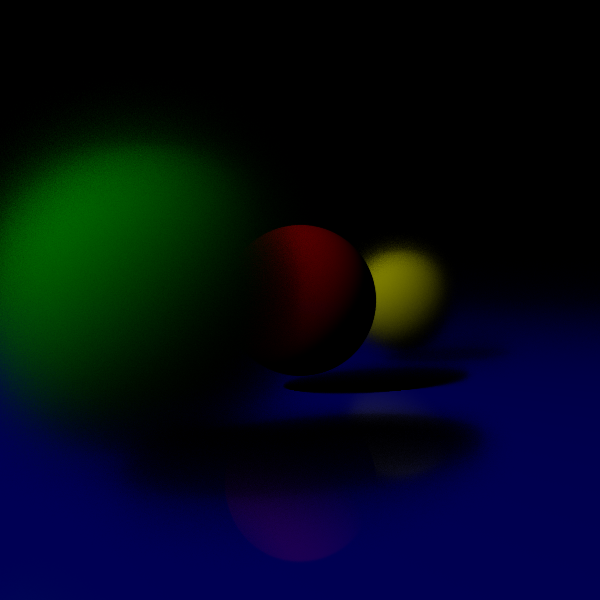
\includegraphics[width=\textwidth, keepaspectratio=true]{../../diary/18.png}
  \caption{Un exemple de rendu de la profondeur de champ avec point de focus
  sur la sphère rouge.}
\end{figure}

\begin{figure}[h]
  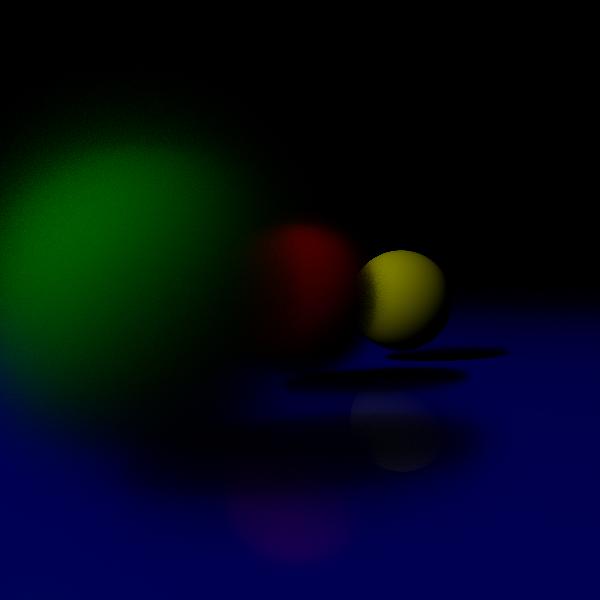
\includegraphics[width=\textwidth, keepaspectratio=true]{../../diary/19.png}
  \caption{Un exemple de rendu de la profondeur de champ avec point de focus
  sur la sphère jaune.}
\end{figure}

\subsection{Amélioration}
\begin{description}
  \item [Meilleur cohérence de l'ouverture] Par analogie avec la photographie,
  le facteur de déviation des rayons lumineux par rapport au centre optique
  est réglé grâce au paramètre \ttt{aperture}. Hélas, ce paramètre devra
  changer en fonction de la taille de la scène car une déviation d'une unité
  dans un monde de 100 unité et un monde de 0.1 unité ne provoque pas du tout
  les même résultat. Il faudrait donc trouver un meilleur paramètre pour ces
  quantité et le définir de manière absolue.
\end{description}

\subsection{Bug connu}
La gestion du focus sur un point situé dans les Z négatifs ne fonctionne pas.
